\documentclass[a4paper, 12pt]{article}
%%\usepackage[italian]{babel}
\usepackage[utf8x]{inputenc}
\usepackage{amssymb}
\usepackage{amsthm}
\usepackage{amsmath}
\usepackage{wrapfig}
\usepackage{titlesec}
\usepackage{multicol}
\usepackage{geometry}
\usepackage{tikz}
\usetikzlibrary{arrows,automata,positioning}
\graphicspath{ {./immagini/} }
\frenchspacing
\newcommand{\subtitle}[1]{%
  \posttitle{%
    \par\end{center}
    \begin{center}\large#1\end{center}
    \vskip0.5em}%
}
\titleformat*{\section}{\Large}
\geometry{a4paper, top=2cm, bottom=2cm, left=2.5cm, right=2.5cm,  heightrounded, bindingoffset=5mm}
\title{Informatica Teorica}
\author{Stefano Staffolani}
\date{ Anno accademico 2022-2023}
\newtheorem{theorem}{Theorem}[section]
\newtheorem{lemma}[theorem]{Lemma}
\newtheorem{corollary}{Corollary}[theorem]
\begin{document}
\maketitle
\tableofcontents
\newpage
\section{Puntate precedenti}
qui metto quello che manca dalle lezioni precedenti....
\section{La macchina di Turing}
Una macchina di Turing \`e una tupla $\langle \sum, Q,q_0,H,\delta\rangle$. Dove: 
\begin{enumerate}
\item $\sum$ \`e un \textbf{alfabeto} di simboli, che include un simbolo speciale $\emptyset$ che indica una cella vuota.
\item $Q$ \`e un insieme finito di \textbf{stati}.
\item $q_0 \in Q$ \`e lo stato iniziale.
\item $H \subset Q$ \`e l'insieme degli \textbf{stati accettanti (o finali)}.
\item $\delta$ \`e la funzione di transizione $\delta: (Q \backslash H) \times \sum \rightarrow Q \times \sum \times \{ \rightarrow, \leftarrow \} $
\end{enumerate}
$\delta$ esprime il programma che governa il funzionamento della TM, ed \`e una funzione totale. Possimao scrivere la definizione di $\delta$ come un insieme di quintuple.
\subsection{Espressivit\`a delle macchine di Turing}
Molto spesso un problema che vogliamo risolvere usando uno strumento di calcolo pu\`o essere espresso come un problema di decisione. Ad esempio\begin{itemize}
\item Dato un grafo, \`e strettamente connesso?
\item Dato un insieme di equazioni, ha una soluzione?
\end{itemize}
\textbf{Come fare tutto ci\`o con delle macchine di Turing?}\\
Abbiamo visto che le TM possono calcolare funzioni di tipo $\mathbb{N}^{k} \rightarrow \mathbb{N}$, il passaggio chiave \`e codificare un probleman di decisione come la $funzione\ caratteristica$ di un $linguaggio\ formale$.
\subsection{Linguaggi formali: ripasso}
Dato un alfabeto $\sum$ di simboli, un \textbf{linguaggio formale} \`e un sottoinsieme di $\sum^{*}$. Ad esempio:
\begin{itemize}
\item Alfabeto $\sum\ =\ \{1\}$
\item Linguaggio delle stringhe di lughezza pari: $L\ =\ \{\epsilon, 11,1111,...\}$
\end{itemize}
La \textbf{funzione caratteristica} di un linguaggio $L$ \`e la funzione \begin{center}
\begin{equation}
\chi_{L}(X) =
	\begin{cases}
		1, & \text{if}\ x \in L \\
      	0, & \text{otherwise}
	\end{cases}
\end{equation}
%$chi_{L}(X)= \Biggl\{ \Biggr\}$
\end{center}
\subsection{Dai problemi di decisione ai linguaggi formali}
Il nostro schema di codifica deve essere tale che dato $\alpha$ (dati del problema di decisione) otteniamo $code(\alpha) \in \sum^{*}$. Il linguaggio che codifica il \textbf{problema di decisione} sar\`a:
\begin{center}
$L\ =\ \{x \in \sum^{*} | x=code(\alpha)\ per\ qualche\  \alpha \land \alpha \in pos(P) \}$\\
Dove $pos(P)$ sono le istanze positive del problema P (dati per i quali la risposta \`e si).
\end{center}
Le propriet\`a\footnote{Quando si guarda alla complessità computazionale, altre proprietà
diventano rilevanti: ad esempio quando la codifica é ridondante e calcolata
in modo efficiente.} che solitamente vogliamo per $code(-)$ sono:
\begin{enumerate}
\item $\alpha \neq \beta \implies\ code(\alpha) \neq code(\beta) $;
\item Dovremmo poter verificare se $x \in \sum^{*}$ \`e $code(\alpha)$ per qualche $\alpha$;
\item Dovremmo poter calcolare $\alpha$ a partire da $code(\alpha)$.
\end{enumerate}
\subsection{Linguaggi decidibili}
\begin{center}
\textbf{Come facciamo a ragionare su un problema di decisione utilizzando una macchina di Turing?}
\end{center}
Assumiamo una codifica del problema di decisione come un linguaggio $L$ su un alfabeto $\sum'$. Vogliamo una Tm $M$ con le seguenti propriet\`a: \begin{enumerate}
\item l'alfabeto di input/output $\sum_{I}$ \`e $\sum'$.
\item l'insieme degli stati finali \`e $H\ =\ \{Y,N\}$.
\end{enumerate}
Diciamo che $M$ \textbf{accetta} un input $x \in \sum_{I}^{*}$ se la computazione ferma in stato $Y$. $M$ \textbf{rigetta} x se ferma in stato $N$.\\
$M$ \textbf{decide} $L$ se:
\begin{itemize}
\item $x \in L \implies\ M\ accetta\ x.$
\item $x \notin L \implies\ M\ rigetta\ x.$
\end{itemize}
Un linguaggio (un problema di decisione) \`e \textbf{decidibile} se c'\`e una TM che lo decide.
\subsection{Linguaggi riconoscibili}
Assumiamo una codifica del problema di decisione come un linguaggio $L$ su un alfabeto $\sum'$. Vogliamo una TM con alfabeto di input/output $\sum'$.\\
$M$ \textbf{riconosce} $L$ se:
\begin{itemize}
\item $x \in L \implies\ M\ si\ ferma$(= raggiunge uno stato finale).
\item $x \notin L \implies\ M\ non\ si\ ferma$(= entra in un ciclo).
\end{itemize}
Un linguaggio (un problema di decisione) \`e \textbf{riconoscibile} se c'\`e una TM che lo riconosce.\\
\begin{center}
$Decidibile \implies Riconoscibile$
\end{center}
\section{WHILE un linguaggio di programmazione di alto livello	}
Turing-completo: quando il suo potere espressivo e' equivalente ad una macchina di Turing. 
Quindi quando qualcuno scrive un nuovo linguaggio deve preoccuparsi del fatto che esso sia Turing-complete.
Non tutti i linguaggi sono Turning-Completi. Ad esempio i domain specific language.
Sintassi in maniera informale:
\begin{enumerate}
\item 1) assegnazione di variabili $X:=3$
\item 2) cicli while   while $X \neq Y$ do Program
\item 3) sequenziamento di programmi  $program1; program2; program3$
\item 4) altri costrutti come $if-then-else$ possono essere definiti a partire da questi primitivi.
\end{enumerate}  1) assegnazione di variabili $X:=3$
NB: NON ci sono $side-effects$(tipo print(42))
\subsection{Semantica}
Un programma WHILE calcola una funzione paziale da $\mathbb{N}^{k} \rightarrow \mathbb{N}$ 
\subsection{Equivalenza}
\begin{theorem}
Una funzione (parziale ) é computabile da un programma WHILE se e solo se é computabile da una macchina di Turing.
\end{theorem}
\begin{proof}
La dimostrazione e` per induzione sulla struttura di un programmma WHILE, supponiamo basato su variabili \(X_1...X_k\)
\begin{enumerate}
\item Caso base
	Se il programma e` un'assegnazione di 0 ad una variabile:
	\(begin X_j := 0 end\) la TM corrispondente e` quella che su input rimpiazza il valore di \(X_j\) con 0.
	Gli altri casi base sono il programma vuoto e le altre due forme di assegnazione.
\item Caso induttivo
	Ci sono due casi da considerare: sequenza e ciclo while.
	\begin{itemize}
	\item sequenza
		per II abbiamo un programma della forma \(begin P_1;P_2;...;P_j end\)
		dove \(P_1,...\) sono programmi per i quali abbiamo, da ipotesi induttiva, TM equivalenti M1,... rispettivamente. La TM per \( begin P_1;...;P_j end\) e` definita nel seguente modo a partire da esse, dove l'output di Mi viene dato come input di Mi+1.
	\item ciclo while
	Assumiamo un programma della forma \(begin while X_{i} != X_j do P end \) dove P e` un programma per il quale, da ipotesi induttiva, abbiamo un aTM M  equivalente. Possiamo costruire una TM \(M_{test}\) che rigetta l'input se il valore di \(X_{i} e X_{j}\) e` diverso, ed accetta altrimenti. La TM per il nostro programma e` costruita come segue: (snapshot da inserire)
	\end{itemize}
\end{enumerate}
\end{proof}

\section{Macchina di Turing Universale}
\subsection{Programmi universali} 
Un programma universale e` un programma pensato per ricevere altri programmi come input ed eseguirli. I sistemi operativi sono esempi di programmi universali.\\
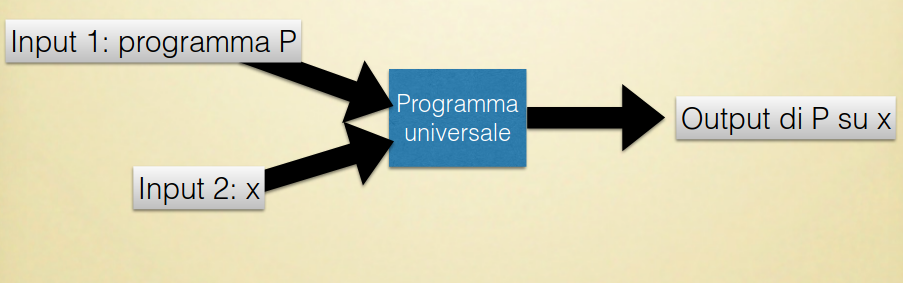
\includegraphics[scale=0.5]{programmi_universali.png}
Anche gli interpreti sono programmi universali.\\
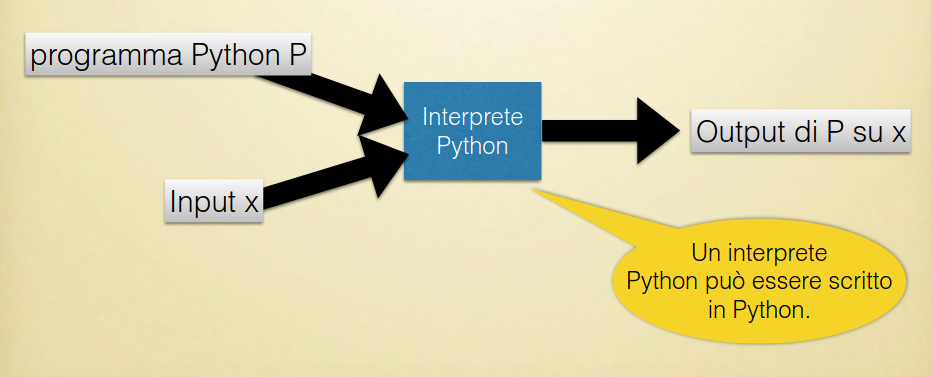
\includegraphics[scale=0.5]{interpreti_programmi_universali.png}
\subsection{La macchina di Turing universale (UTM)}
La UTM prende in input una stringa y, e per prima cosa verifica che y sia della forma code(M)code(x), dove code() e` una codifica, M e` un TM, e x una stringa nell'alfabeto di input \(\sigma_i di M.\)
Se e` cosi`, allora la UTM simula l'esecuzione di M siu x.\\ 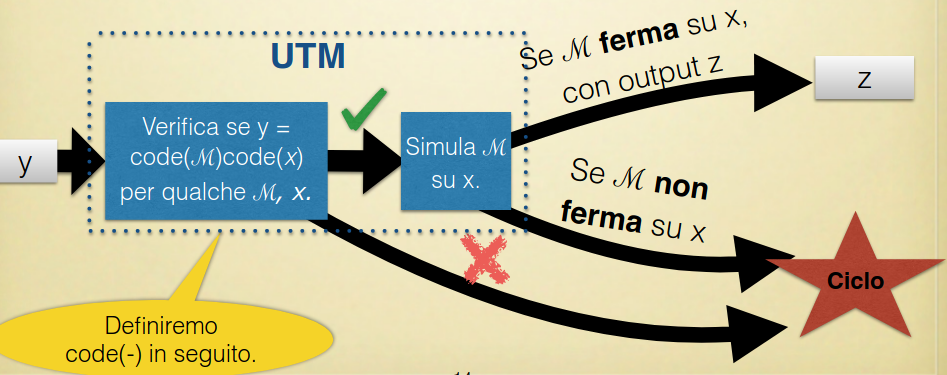
\includegraphics[scale=0.5]{UTM.png}
\subsection{Codificare una TM}
\(M = (\sigma, Q, q_0, H, \delta)\)
Introduciamo alcune convezioni. Gli stati in Q sono ordinati come \(q_0,q_1,...\) con \(q_0\) iniziale. Ordiniamo i simboli che possono apparire nella definizione di \(\delta\)
\[\sigma0 = \emptyset \   \ \sigma1 = \rightarrow \    \ \sigma2=\leftarrow \]
e gli altri simboli in \(\sigma\) come \(\sigma4,..\)
Possiamo codificare gli stati ed i simboli come stringhe unarie: \[code(q_i) = 11...1 \   \ code(\sigma_i)=11...1\]
Codifichiamo una tupla t di $\delta$ come: \[code(t) =code(q_i)0code(\sigma_n)0code(q_j)0code(\sigma_m)0code(\sigma_0)0\]
E la funzione di transizione $\delta={t_1,t_2,...,t_k}$ come \[code(\delta) = code(t_1)0code(t_2)0...0code(t_k)0\]
Possiamo dedurre quali sono gli stati finali di H: sono quelli su cui $\delta$ non e` definita (= non occorrono mai in terza posizione in una tupla).
INSERIRE ESEMPIO
\subsection{Osservazioni sulla codifica}
E` possibile che ci siano due o piu' TM che computino la stessa funzione, ma codificate come stringhe differenti (intuitivamente: se esprimono un diverso algoritmo). Nondimeno, la codifica e` \(iniettiva\): due macchine differenti saranno codificate da stringhe differenti. Data una stringa su {0,1}, e` possibile determinare se sia o meno il codice di una TM (e di quale). In particolare: si tratta di un problema \textbf{decidibile}.\\
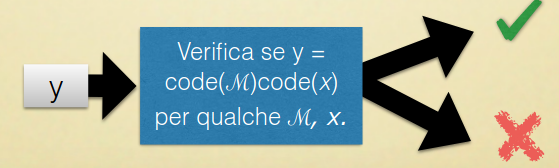
\includegraphics[scale=0.6]{codifica_UTM.png}

\subsection{Costruzione di una UTM}
La UTM e` definita come una macchina di Turing con tre nastri. 
\begin{enumerate}
\item Nastro 1 mantiene il nastro di M in forma codificata.
\item Nastro 2 manterra` code(M).
\item Nastro 3 manterra` o stato corrente di M in forma codificata.
\end{enumerate}
Un passo della simulazione di  M da parte della UTM funziona nel seguente modo.
\begin{enumerate}
\item Cerca in code(M) una tupla $⟨ q_i, \sigma_n, q_j, \sigma_m, \sigma_o ⟩$ dove qi concida con lo stato sul nastro 3 e $\sigma_n$ coincida con il simbolo attualmente esaminato da M.
\item Aggiorna nastro 1 con il nuovo simbolo $\sigma_0$ e sposta la testina nella direzione $\sigma_m$.
\item Aggiorna nastro 3 con lo stato $q_j$. Se é finale, fermati.
\end{enumerate}
\subsection{Considerazioni finali}
Questa costruzione mostra l'esistenza di una macchina di Turing universale, $M_U$. Niente impedisce a $M_U$ di ricevere la sua stessa codifica code($M_U$) come parte dell'input! Questa forma di autoreferenzialita` sara` utilizzata nella prossima lezione per dimostrare che esiste un problema indecidibile.

\section{Cosa non possono fare le TM}
Introduciamo il nostro primo problema indecidibile: il problema della \textbf{fermata}($halting\ problem$). Questo risultato ci informa, pi\`u in generale, sui limiti della computazione per algoritmi. Abbiamo visto che l'essere calcolabile da una procedura algoritmica implica essere calcolabile da una TM. Dunque \textbf{non} essere calcolabile da una TM implica non essere calcolabile da nessuna procedura algoritmica.
\subsection{Ripasso: Linguaggi e TM}
\begin{theorem}
Una TM $M$ \textbf{decide} un linguaggio \textbf{L} se:
\begin{enumerate}
\item Quando $x \in L$, allora $M$ accetta $x$(= ferma nello stato Y).
\item Quando $x \notin L$, allora $M$ rigetta $x$(= ferma nello stato N).
\end{enumerate}
\end{theorem}

\begin{theorem}
Una TM $M$ \textbf{riconosce} un linguaggio \textbf{L} se:
\begin{enumerate}
\item Quando $x \in L$, allora $M$ termina.
\item Quando $x \notin L$, allora $M$ non termina.
\end{enumerate}
\end{theorem}
\subsection{Gradi di (in)calcolabilit\`a}
\begin{enumerate}
\item Decidibile da una TM se e solo se \`e calcolabile($\exists$ un algoritmo che risponde "Si" o "No").
\item Non decidibile da nessuna TM ma riconoscibile da una qualche TM se e solo se non \`e calcolabile(Semi-decidibile: nessun algoritmo sapr\`a calcolare tutte le risposte "No").
\item Non riconoscibile da nessuna TM se e solo se non \`e calcolabile(del tutto non calcolabile: qualsiasi algoritmo fallir\`a nel dare sia le risposte "Si" che "No").
\end{enumerate}
\subsection{Un problema indecidibile: Halting Problem}
Supponiamo che esista un a codifica $code(-)$ che presa una TM su alfabeto $\sum$ restituisce le stringhe $x \in \sum^*$. La codifica usata per definire la macchina di Turing universale \`e un esempio di tale procedura.
Definiamo il linguaggio del \textbf{problema della fermata}:
\begin{center}
HALT = \{(y,x) $\in \sum^*$x$\sum^*|$ y = code($M$) $e$ $M$ ferma su x. \}
\end{center} 
\begin{theorem}
\label{th:1}
Il problema della fermata \`e riconoscibile ma non \`e decidibile.
\end{theorem}
\begin{proof}
Dimostriamo che HALT \`e riconoscibile$^{[1]}$ e che non \`e decidibile$^{[2]}$.\\
\begin{enumerate}
\item Dimostriamo che HALT \`e riconoscibile. Dobbiamo costruire una TMU $M_H$ che prende in input una coppia $(y,x)$, se $y$ ferma su $x$ $M_H$ si ferma altrimenti cicla.
\item dimostriamo che HALT non \`e decidibile. Assumiamo che HALT sia decidibile, e chiamiamo $M_H$ la TM che decide HALT. Perci\`o $M_H$ si comporter\`a come segue. Se $y=code(M)$ per un qualche $M$: \\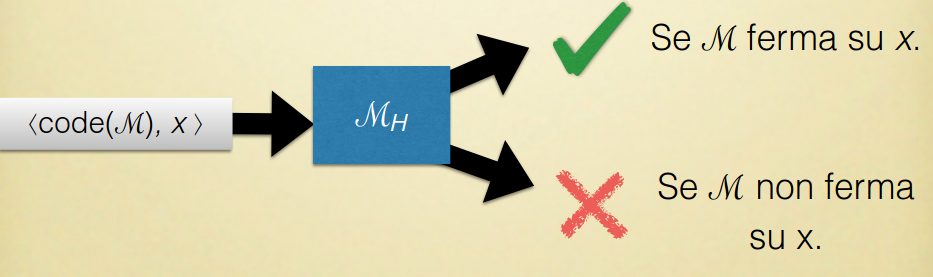
\includegraphics[scale=0.4]{TM_HALT1.png}\\
Possiamo definire una nuova TM $M'$ come segue.\\ 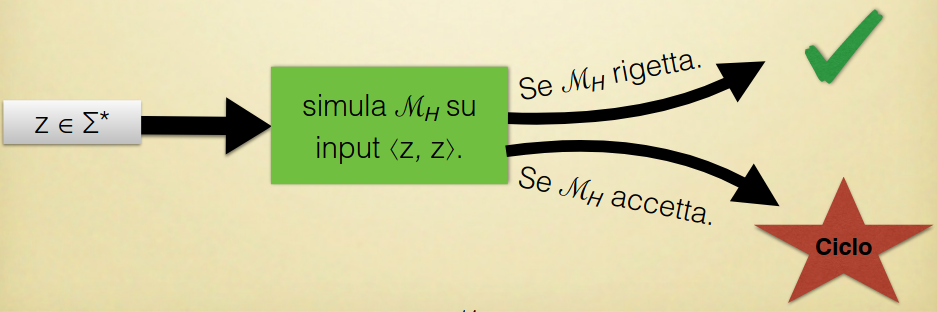
\includegraphics[scale=0.4]{TM_HALT2.png}\\
Proviamo ora ad  eseguire $M'$ su input $code(M')$.\\ 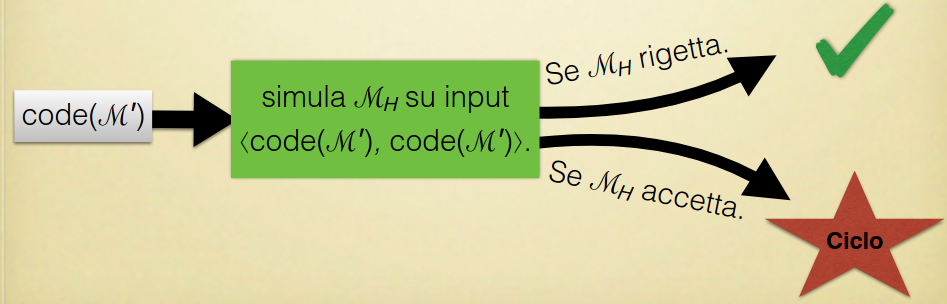
\includegraphics[scale=0.4]{TM_HALT3.png}
\\Dunque \\
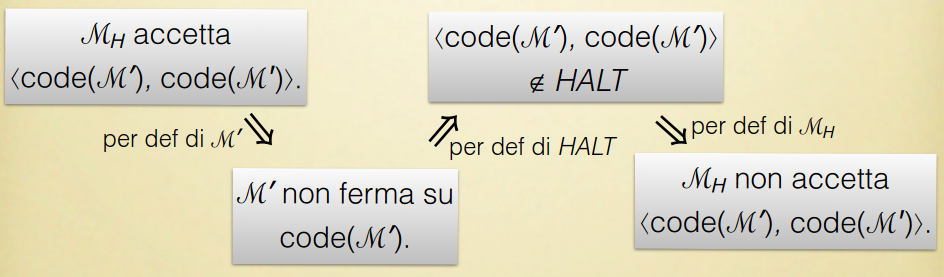
\includegraphics[scale=0.4]{HALT4.png}\\
Contraddizione. Proviamo il caso in cui rigetta.\\
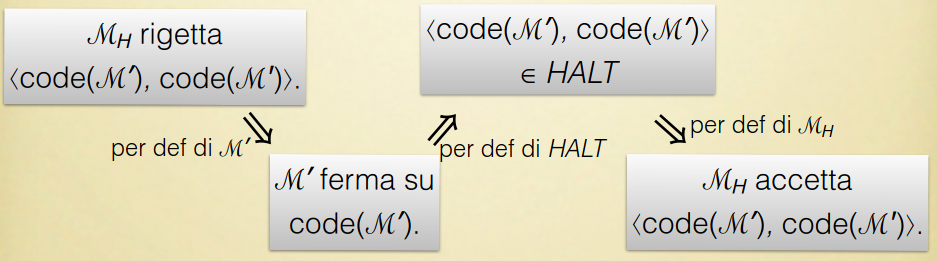
\includegraphics[scale=0.4]{HALT5.png}\\
Anche questo caso \`e in contraddizione. L'unica assunzione utilizzata nel costruire $M'$ \`e che $\exists M_H$ che decide HALT. Perci\`o $M_H$ non pu\`o esistere: HALT \`e indecidibile.
\end{enumerate}
\end{proof}

\subsection{Problemi non riconoscibili}
\begin{theorem}
Il complemento $HALT^{-}$ del problema della fermata non \`e riconoscibile da nessuna TM.
\begin{center}
$HALT$ = \{$\langle y,x \rangle \in \sum^{*}x\sum^{*}|$ y=code($M$) e $M$ ferma su x.\}
\end{center}
\begin{center}
$HALT^{-}$ = \{$\langle y,x \rangle \in \sum^{*}$x$\sum^{*}|$ y $\neq$ code($M$) $\forall$ $M$ o y=code($M$) e $M$ non ferma su x\}
\end{center}
\end{theorem}
C'\`e una dimostrazione diretta, per contaddizione, ma \`e pi\`u interessante mostrare una dimostrazione pi\`u astratta. Deriva dal seguente teorema.
\begin{theorem}
Se $HALT^{-}$ fosse riconoscibile, allora HALT sarebbe decidibile.
\end{theorem}
%Infatti, dal momento che HALT \`e indecidibile, se questo teorema \`e varo allora $HALT^{-}$ non pu\`o essere riconoscibile.
\begin{proof}
Abbiamo gi\`a visto che HALT \`e riconoscibile, diciamo da una TM $M_{HR}$. Supponiamo per assurdo che anche $HALT^{-}$ sia riconoscibile, e chiamiamo $M_{H^{-}}$ la TM che lo riconosce. Possimao ora costruire una TM $M_H$ che decide HALT come segue. Su input $\langle y,x \rangle$, simula $M_{HR}$ e $M_{H^{-}}$ in parallelo su input $\langle y,x \rangle$. Se $M_{HR}$ ferma, accetta. Se $M_{H^{-}}$ ferma, rigetta.\\
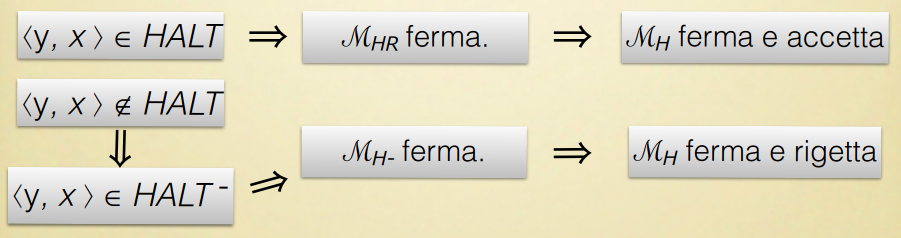
\includegraphics[scale=0.4]{TM_complemento_HALT.png}\\
Perci\`o $M_H$ decide HALT.
\end{proof}
Dal momento che HALT \`e indecidibile, allora $HALT^-$ non pu\`o essere riconoscibile.
\subsection{Osservazione 1. Complemento linguaggio riconoscibile}
La dimostrazione data non sfruttaa in alcun modo il fatto che HALT sia definito nel modo in cui \`e definito" potremmo sostituire HALT con qualsiasi problema riconoscibile, e funzionerebbe lo stesso. Abbiamo dunque il seguente teorema.
\begin{theorem}
\label{th:2}
Se $L$ e $L^{-}$ sono riconoscibili, allora $L$ \`e decidibile.
\end{theorem}
\begin{proof}
La stessa data per $L = HALT$
\end{proof}
Dai teoremi \ref{th:1} e \ref{th:2} otteniamo il seguente corollario.
\begin{corollary}
I linguaggi riconoscibili non sono chiusi sotto complemento.
\end{corollary}
\begin{proof}
HALT \`e riconoscibile ma il suo complemento non \`e riconoscibile.
\end{proof}
\subsection{Osservazione 2. Ridurre un problema ad un altro}
La nostra dimostrazione del fatto che $HALT^{-}$ non sia riconoscibile ha la seguente struttura:
\begin{center}
Se potessimo riconoscere L, allora potremmo decidere L'.\\ Poich\`e non \`e decidibile, allora non possiamo riconoscere L.
\end{center}
Come ridurre L a L'? Vedremo come questa intuizione possa essere formalizzata in una tecnica di dimostrazione, che ci permette di ridurre problemi tra di loro al fine di dimostrarne la non calcolabilit\`a.
\section{esercitazione 1 Marzo 2023}
\subsection{Quesito 1}
Un problema che vogliamo risolvere usando uno strumento di calcolo puo' essere espresso come un problema di decisione. Questi problemi hanno la componente dei dati e la risposta SI/NO. Per poter risolvere questi problemi con un calcolatore e' necessario codificare un problema di decisinoe come la funzione caratteristica di un linguaggio formale.

Dato a e b dati le cui codifiche sono code(a) e code(b) $\in \sum^*$
Le proprieta' che la codifica deve rispettare sono: 
\begin{enumerate}
\item $a \ne b \ code(a) \neq code(b)$
\item deve essere verificabile che se x $\in \sum^*$ \`e $code(a)$ per qualche $a$
\item deve essere calcolabile a partire da $code(a).$
\end{enumerate}
\subsection{Problema 2.1}
Alfabeto $\sum = \{0,1\}$
La TM deve accettare l'input quando esso contiene 101 e rifiutare altrimenti.\\
\begin{tikzpicture}[shorten >=2pt,node distance=4cm,auto, on grid]

  \node[state,initial]   (1)  {$q_0$};
  \node[state, yshift=-1cm] (2) [right=of 1]  {$q_1$};
  \node[state, yshift=1cm] (3) [right=of 2]  {$q_2$};
  \node[state,accepting] (4) [right=of 3]  {$Y$};
  \node[state,accepting] (5) [below=of 2]	{$N$};

  \path[->]
  	(1) edge [loop above] node {$0,0,\rightarrow$} (1)
  	(1) edge [bend right] node {$\emptyset,\emptyset,\rightarrow$} (5)
	(1) edge  node {$1,1,\rightarrow$} (2)
	(2) edge [loop above] node {$1,1,\rightarrow$} ()  	
  	(2) edge  node {$\emptyset,\emptyset,\rightarrow$} (5)
  	(2) edge  node {$0,0,\rightarrow$} (3)
  	(3) edge [] node {$1,1,\rightarrow$} (4)
  	(3) edge [bend right, above] node {$0,0,\rightarrow$} (1)
  	(3) edge [bend left] node {$\emptyset,\emptyset,\rightarrow$} (5)
  	;
  	
\end{tikzpicture}

\subsection{Problema 2.2}
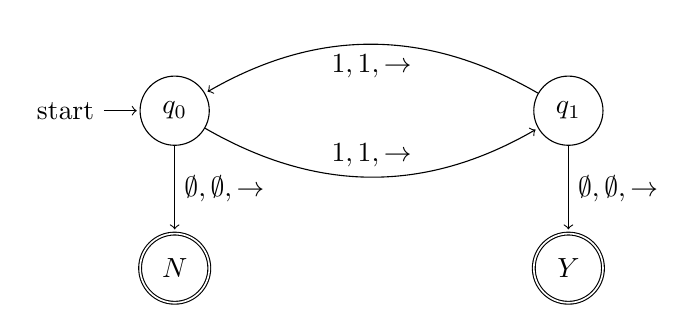
\begin{tikzpicture}[shorten >=1pt,node distance=5cm,auto, on grid]
	\node [state, initial] (1) {$q_0$};
	\node [state] (2) [right=of 1] {$q_1$};
	\node [state, accepting, yshift=3cm] (3) [below=of 1] {$N$};
	\node [state, accepting, yshift=3cm] (4) [below=of 2] {$Y$};
	
	\path[->]
		(1) edge [bend right] node  {$1,1,\rightarrow$} (2)
		(2)	edge [bend right] node  {$1,1,\rightarrow$} (1)
		(1) edge node  {$\emptyset,\emptyset,\rightarrow$} (3)
		(2) edge node  {$\emptyset,\emptyset,\rightarrow$} (4)
		;

\end{tikzpicture}

\section{Mapping-reduction}
Abbiamo dimostrato che 
\begin{enumerate}
\item il problema della fermata ($HALT$) \`e indecidibile.
\item Il complemento del problema della fermata ($HALT^{-}$) non \`e riconoscibile. Questo pu\`o essere dimostrato come conseguenza del punto 1.
\end{enumerate}
Introduciamo dunque una tecnoca semplice e generale per dimostrare l'indecidibilit\`a/non-riconoscibilit\`a di un problema: \textbf{mapping-reduction}.\\
Questa tecnica ci consente di $ridurre$ le istanze di un problema a quelle di un altro problema. Nel confrontare due problemi la \textbf{decidibilit\`a/riconoscibilit\`a non \`e essenziale nel processo di prova}. Pu\`o essere derivata come una conseguenza.
\subsection{Perch\`e}
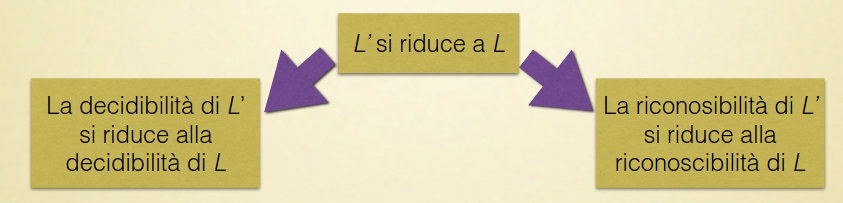
\includegraphics[scale=0.5]{mapred1.png}\\
Rispetto ad un tentativo di investigare la calcolabilit\`a di $L$ o $L'$, questo approccio \`e maggiormente strutturato: ci consentriamo sulla relazione dei problemi.
\subsection{Definizione}
Siano $L$ e $L'$ linguaggi sull'alfabeto $\sum$, diciamo che $L'$ \`e $mapping-riducibile$ a $L$, scritto $L' \leq L$, se esiste una TM che computa la funzione (totale) $f: \sum^* \rightarrow \sum*$ tale che 
\begin{center}
$x \in L' \iff f(x) \in L$
\end{center}
Sostanzialmente, $f$ converte il problema di appartenenza per $L'$ nel problema di appartenenza per $L$. Intutivamente $L' \leq L$: $L$ \`e difficile almeno quanto $L'$.
\subsection{Riduzione e Decidibilit\`a}
La mapping-reducibility non parla di decidibilit\`a. \`E per\`o uno strumento efficace per mostrare che un linguaggio \`e (in)decidibile.
\begin{theorem}
\label{th:4}
Se $L' \leq L$ e $L$ \`e decidibile, allora $L'$ \`e decidibile.
\end{theorem}
\begin{corollary}
Da \ref{th:4} se $L' \leq L$ e $L'$ \`e indecidibile, allora $L$ \`e indecidibile. Quindi, per dimostrare che $L$ \`e indecidibile, \`e sufficiente mostrare che $HALT \leq L$.
\end{corollary}
\begin{corollary}
Da \ref{th:4} se $L$ \`e decidibile e $L'$ non lo \`e, allora $L' \nleq L$.
\end{corollary}
\subsection{Mapping-reduction in azione: ETH}
Il problema della fermata su nastro vuoto ($ETH$) \`e definito dal linguaggio:
\begin{center}
$ETH = \{x \in \sum^* | x = code(M) \land M ferma\ su\ \epsilon\}$
\end{center}
\begin{theorem}
\label{th:5}
ETH \`e indecidibile.
\end{theorem}
Idea della dimostrazione: ridurre $HALT$ a $ETH$, cos\`i che l'indecibilit\`a di $HALT$ implichi quella di $ETH$, grazie a \ref{th:4}.
\begin{proof}
Costruiamo una funzione computabile $f$ tale che:
\begin{center}
$\langle y,x \rangle \in HALT \iff f(\langle y,x \rangle) \in ETH$
\end{center}
La definizione di $f$ \`e come segue. Su argomento $\langle y,x \rangle$:
\begin{itemize}
\item Se $\forall M.y \neq code(M)$ allora $f(\langle y,x \rangle) = y \neq ETH$.
\item Se $y=code(M)$, allora $f(\langle y,x \rangle) = code(M_{M,x})$ \`e costruita come segue:
\begin{enumerate}
\item $M_{M,x}$ entra in loop su oni stringa non vuota ($\neq \epsilon$).
\item su input $\epsilon$, scrive $x$ sul nastro e simula $M$ su $x$.\\
\end{enumerate}
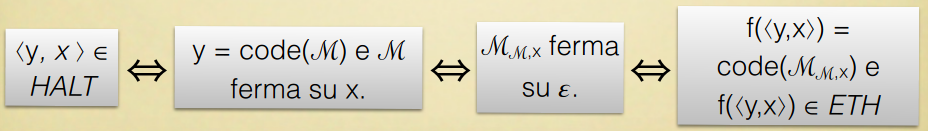
\includegraphics[scale=0.4]{ETH1.png}
\end{itemize}
\end{proof}
\subsection{Il full language problem}
Il "full language" problem ($FL$) \`e definito dal linguaggio seguente:
\begin{center}
$FL = \{x \in \sum^* | x=code(M) \land M ferma\ su\ ogni\ input\}$
\end{center}
\begin{theorem}
$FL$ \`e indecidibile.
\end{theorem}
Schema della dimostrazione: Riduciamo $HALT$ a $FL$.
\begin{proof}
Costruiamo una funzione $f$ computabile tale che: 
\begin{center}
$\langle y,x \rangle \in HALT \iff f(\langle y,x \rangle) \in FL$
\end{center}
Definiamo $f$ come segue. Su argomento $\langle y,x \rangle$:
\begin{itemize}
\item Se $\forall M.y \neq code(M)$, allora $f(\langle y,x \rangle) = y \in FL$.
\item Se $y =code(M)$, allora $f(\langle y,x \rangle) = code(M_{M,x})$, dove $M_{M,x}$ \`e costruita come segue:
\begin{enumerate}
\item $M_{M,x}$ cancella il suo input.
\item scrive $x$ sul nastro e simula $M$ su $x$.
\end{enumerate}
\end{itemize}
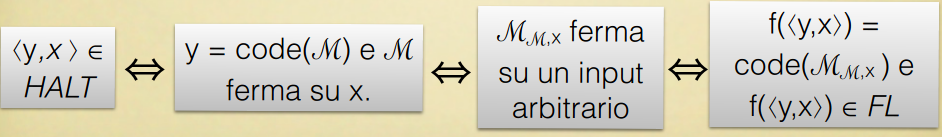
\includegraphics[scale=0.45]{FL1.png}\\
\end{proof}
\subsection{L'equivalence problem}
L'\textbf{equivalence problem} (EQ) per le TM \`e definito dal seguente linguaggio:
\begin{center}
$EQ = \{\langle y,x \rangle \in \sum^{*}\times\sum^{*} | x=code(M),y=code(M') \land f_{M} = f_{M'}\}$\\
Ovvero $M$ e $M'$ computano la stessa funzione parziale.
\end{center}
\begin{theorem}
$EQ$ \`e indecidibile.
\end{theorem}
Idea della dimostrazione: Riduciamo $FL$ a $EQ$.\footnote{Osserva che avremmo potuto usare la riduzione da $HALT$, abbiamo cambiato per mostrare la flessibilit\`a di questo approccio.}
\begin{proof}
\`E sufficiente costruire una funzione computabile $f$ tale che:
\begin{center}
$z \in FL \iff f(z) \in EQ$
\end{center}
La definizione di $f$ \`e come segue. Su argomento $z$:
\begin{itemize}
\item $\forall M. z \neq code(M) \implies f(z) = \langle z,z\rangle \notin EQ$.
\item $z=code(M) \implies f(z) = \langle code(M_1), code(M_2) \rangle$, dove $M_1$ e $M_2$ sono definite coem segue:
\begin{enumerate}
\item $M_1$ esegue $M$ sul suo input e restituisce 1 se $M$ si ferma, e va in loop altrimenti.
\item $M2$ restituisce 1 $\forall input$.
\end{enumerate}
\end{itemize}
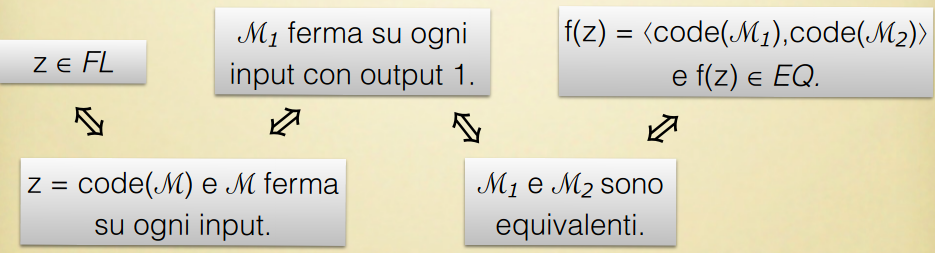
\includegraphics[scale=0.5]{EQ1.png}\\
\end{proof}
\subsection{Riduzione e Riconoscibilit\`a}
Ci\`o che \`e vero per riduzione e decidibilit\`a vale anche per riduzione e riconoscibilit\`a.
\begin{theorem}
\label{th:6}
Se $L' \leq L \land L$ \`e riconoscibile $\implies L'$ \`e riconoscibile.
\end{theorem}
\begin{corollary}
Da \ref{th:6} $L' \leq L \land L'\ $ non \`e riconoscibile $\implies L$ non \`e riconoscibile.
\end{corollary}
\begin{corollary}
Da \ref{th:6} Se $L$ \`e riconoscibile $\land L'\ $ non lo \`e $\implies L' \nleq L$. 
\end{corollary}
\subsection{l'equivalence problem non \`e riconoscibile}
Abbiamo dimostrato che $EQ$ \`e indecidibile. Ora mostriamo che $EQ$ non \`e riconoscibile. Ricordando che $EQ$ \`e definito come segue:
\begin{center}
$EQ = \{\langle y,x \rangle \in \sum^{*}\times\sum^{*} | x=code(M),y=code(M') \land f_{M} = f_{M'}\}$\\
Ovvero $M$ e $M'$ computano la stessa funzione parziale.
\end{center}
\begin{theorem}
\label{th:7}
$EQ$ non \`e riconoscibile.
\end{theorem}
Idea della dimostrazione: Riduciamo $HALT^{-}$ (che sappiamo essere un problema non-riconoscibile) a $EQ$.
\begin{proof}
Ricordiamo la definizione di $HALT^{-}$:
\begin{center}
$HALT^{-} = \{\langle y,x \rangle \in \sum^{*} \times \sum^{*} | \forall M. y \neq code(M) \lor y=code(M) \land M$ non ferma su$x\}$
\end{center}
Per la riduzione, abbiamo la funzione $f$ \begin{center}
$\langle y, x \rangle \in HALT^{-} \iff f(\langle y,x\rangle) \in EQ$
\end{center}
equivalente a \begin{center}
$\langle y,x \rangle \in HALT \iff f(\langle y,x \rangle) \in EQ^{-}$
\end{center}
Su $\langle y,x\rangle$ definiamo $f$ come segue:
\begin{itemize}
\item Se $\forall M. y \neq code(M)$ allora prendiamo $M'$ quialsiasi e consideriamo \\$f(\langle y, x \rangle) = \langle code(M'), code(M)\rangle$.
\item altrimenti $y = code(M)$ e consideriamo $f(\langle y,x \rangle) = \langle code(M_1), code(M_2) \rangle$, dove $M_1$ e $M_2$ sono definite come:
\begin{enumerate}
\item $M_1$ esegue $M$ su $x$ e si ferma se $M$ si ferma, altrimenti entra in un ciclo.
\item $M_2$ entra in un ciclo su ogni input.\\
\end{enumerate}
\end{itemize}
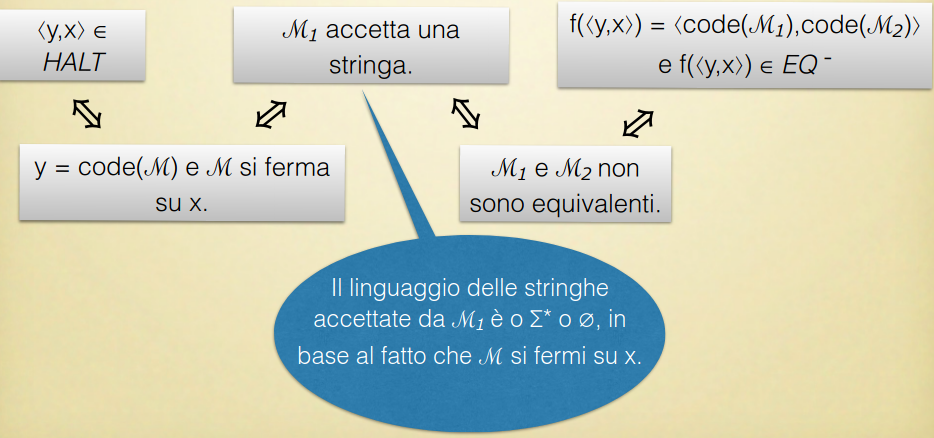
\includegraphics[scale=0.4]{EQ2.png}\\
\end{proof}
\subsection{Ulteriori propriet\`a della mapping-reduction}
\begin{theorem}
\label{th:8}
Se $L' \leq L \land L$ \`e decidibile, allora $L'$ \`e decidibile.
\end{theorem}
\begin{corollary}
Da \ref{th:7} se $L' \leq L \land L'$ \`e indecidibile, allora $L$ \`e indecidibile.
\end{corollary}
\begin{corollary}
Da \ref{th:7} se $L$ \`e decidibile e $L'$ no, allora $L' \nleq L$.
\end{corollary}
Se $L'$ \`e decibile, la riduzione a qualche $L$ \`e di scarsa utilit\`a.
\begin{theorem}
\label{th:9}
Se $L$ \`e un linguaggio non-triviale $(L \neq \sum^{*} \land L \neq \emptyset)$, allora $\forall L'$ decidibile$.L' \leq L$.
\end{theorem}
\begin{proof}
Poich\`e $L$ \`e non-triviale, possiamo prendere $x \in L \land y \notin L$. Definiamo la funzione $f: \sum^{*} \rightarrow \sum^{*}$ come segue:
\begin{enumerate}
\item $f(z) = x$ se $z \in L'$
\item $f(z) = y$ altrimenti 
\end{enumerate}
Poich\`e \`e decidibile, $f$ pu\`o essere implementata tramite una TM che simula internamente la TM per $L'$ e restituisce $x$ o $y$ coerentemente. Inoltre, per definizione di $f$: \begin{center}
$z \in L' \iff f(z) \in L$
\end{center}
\subsection{Riduzione come Relazione}
La riduzione \`e una relazione tra linguaggi.\begin{enumerate}
\item \`E \textbf{riflessiva}: $\forall L. L \leq L'$.
\item \`E \textbf{transitiva}" $L' \leq L \land L \leq L''  \implies L' \leq L''$.
\item Non \`e per\`o \textbf{simmetrica} (sarebbe simmetrica se $L' \leq L \implies L \leq L'$)\footnote{Il problema della fermata \`e un controesempio, per per \ref{th:8} $\forall L'$ decidibile, $L' \leq HALT$, se anche $HALT \leq L'$, allora anche $HALT$ sarebbe decidibile per \ref{th:7}. Contraddizione.} 
\end{enumerate}
Quindi, la riduzione non \`e una relazione di equivalenza. 
\end{proof}
\subsection{Riduzione e Complemento}
\begin{theorem}
\label{th:10}
$L_1 \leq L_2 \iff L_{1}^{-} \leq L_{2}^{-}$.
\end{theorem}
\begin{corollary}
Da \ref{th:9} $L_{1}^{-} \leq L_2 \iff L_1 \leq L_{2}^{-}$.\footnote{Usato implicitamente nella prova di \ref{th:7} con $L_1 = HALT$ e $L_2= EQ$}
\end{corollary}
Mettendo insieme questi risultati, abbiamo senza ulteriore lavoro una prova che $EQ^{-}$ non \`e riconoscibile. Infatti, $HALT \leq FL \leq EQ$, quindi $HALT^{-} \leq EQ^{-}$ per teorema. La non-riconoscibilit\`a di $HALT^{-}$ implica non-riconoscibilit\`a di $EQ^{-}$.
\subsection{Gerarchia dei problemi}
\begin{enumerate}
\item Decidibile.
\item Indecidibile, ma riconoscibile (es. $HALT$).
\item Non riconoscibile, ma il cui complemento \`e riconoscibile (es. $HALT^{-}$).
\item Non riconoscibile, e non il cui complemento non \`e riconoscibile (es. $EQ$).
\end{enumerate}
\subsection{Turing-riducibilit\`a}
La mapping-reducibility è solo uno dei modi in cui definire il concetto di problema riducibile a un altro problema. Un altro \`e la Turing-riducibilit\`a. Un \textbf{oracolo} per il linguaggio $L$ \`e uno strumento esterno ("black box") capace di rispondere alla domanda $"x \in L?" \forall x$.\\ Un linguiaggio $L'$ \`e \textbf{Turning-riducibile} a $L$ se, dato un oracolo per $L$, possiamo decodere $L'$.
\begin{center}
$mapping-riducibility \implies Turing-riducibility$.
\end{center}
Ad esempio sappiamo che $HALT^{-} \nleq HALT$, cio\`e $HALT^{-}$ non \`e mapping-riducibile a $HALT$. MA $HALT^{-}$ \`e Turing-riducibile ad $HALT$. Infatti, se abbiamo un oracolo per la domanda $"\langle y,x \rangle \in HALT?"$, questo pu\`o essere usato per decidere se $\langle y,x \rangle \in HALT^{-}$.
\section{La cardinalit\'a dei problemi irrisolvibili}
\subsection{Obiettivo}
Vogliamo mostrare cjhe la maggior parte dei linguaggi non sono riconoscibili (e, quindi indecidibili). Il nostro argomento consiste nel mostrare che ci sono $"molti"$ pi\`u linguaggi che TM.
\subsection{Insiemi infiniti numerabili}
Un insieme $S$ \`e \textbf{infinito numerabile} se c'\`e una funzione totale biettiva $f: \mathbb{N} \rightarrow S$.
Ad esempio: l'insieme dei numeri dispari $D$ con la funzione $f: \mathbb{N} \rightarrow D$ definita come $f(n) = 2n - 1$.
\begin{lemma}
\label{lemma:1}
Se $S_1$ e $S_2$ sono infiniti numerabili, $S_{1} \cup S_{2}$ \`e infinito numerabile.
\end{lemma}
Ad esempio prendiamo l'insieme $\sum^{*}$ di stringhe su alfabeto finito $\sum$.\\Assumi $|\sum|=n$, la biezione con $\mathbb{N}$ \`e costruita come:
\begin{center}
$f: \mathbb{N} \rightarrow \sum^{*}$
\begin{enumerate}
\item $f(\epsilon) = 1$
\item $\forall i \in \{1..n\}.\ f(\sigma_{i}) = i + 1$
\item $\forall i \in \{1..n\} \forall j \in \{1..n\}.\ f(\sigma_{i} \sigma_{j})= n \times i + i+ j$
\item ecc. per stringhe con lunghezza $> 2$.
\end{enumerate}
\end{center}
Abbiamo visto che ogni TM pu\`o essere codificata come una stringa per un alfabeto $\sum$ con $|\sum| = 2$ (es. $\sum = \{0,1\}$).\\
Allora, l' \textbf{insieme di tutte le TM} \`ee inifinito numerabile. Anche l' \textbf{insieme di tutti i linguaggi riconoscibili} \`e infinito numerabile. Questo perch\`e, per definizione, un linguaggio \`e riconoscibile se c;\`e una TM che lo riconosce. Per la stessa ragione, l' \textbf{insieme delle funzioni} $\mathbb{N} \rightarrow \mathbb{N}\ computabili$ da una TM \`e infonoto numerabile. 
\section{Linguaggi sono non numerabili}

%%%%%%%%%
Sia $S_{\sum}$ l'insieme di tutti i linguaggi sull'alfabeto finito $\sum$.
\begin{theorem}
L;insieme $S_{\sum}$ non \`e numerabile.
\end{theorem}
\begin{proof}
Ricorda che un linguaggio L \`e un sottoinsieme di $\sum^*$. Abbiamo gi\`a visto che $\sum^*$ \`e infinito numerabile, quindi possiamo scriverlo come $\sum^* = \{\sigma_1, \sigma_2,\sigma_3,...\}$. Allora un linguaggio, diciamo $L_1 = \{\sigma_1,\sigma_4\}$, pu\`o essere rappresentato come una riga in una tabella:\\
\begin{center}
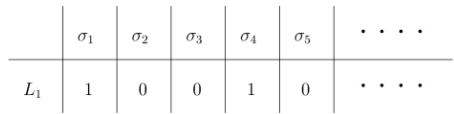
\includegraphics[scale=0.5]{tabella_linguaggi.png}

\end{center}
\end{proof}
Ciascun linguaggio su $\sum$ pu\`o essere rappresentato in questo modo. Per contaddizione, assumi che $S_{\sum}$ sia un insieme numerabile. Allora possiamo assegnare un numero naturale ai suoi elementi, cos\`i che ogni $L_i \in S_{\sum}$ appare come riga a destra.\\ \begin{center}
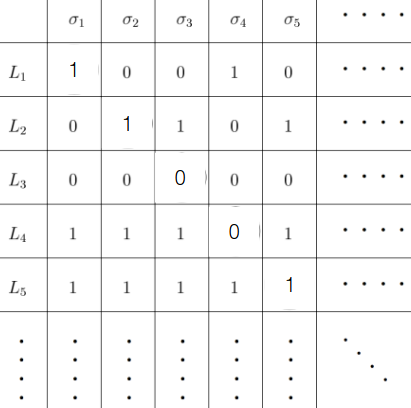
\includegraphics[scale=0.5]{tabella_linguaggi2.png}
\end{center}
Davvero ogni elemento $L$ di $S_{\sum}$ compare su una riga?\\
Definisci $L$ come $00110...$, allora $\sigma_i \in L \iff \sigma_i \notin L_i$. Quindi $L$ \`e diverso da ogni linguaggio $L_i$ sulla riga. Dunque $L$ non pu\`o essere in una riga! \textbf{Contraddizione}.\\ Quindi, $S_{\sum}$ non \`e numerabile.\\ \begin{center}
 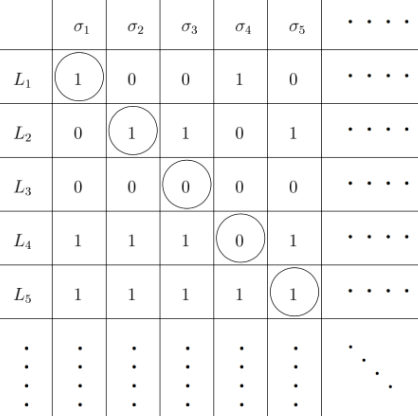
\includegraphics[scale=0.5]{tabella_linguaggi3.png}
\end{center}
\subsection{Riassumendo}
Dato un alfabeto finito $\sum$, abbiamo visto che:
\begin{enumerate}
\item l'insieme di linguaggi riconoscibili da una TM \`e infinito numerabile.
\item l'insieme di tutti i linguaggi \`e non-numerabile.
\end{enumerate}
Quindi, esistono limguaggi che non sono riconoscibili da alcuna TM, ad esempio $HALT^{-}, EQ, EQ^{-}$.\\
\subsubsection{Quanti linguaggi non riconoscibili ci sono?}
La risposta deriva da un  un risultato generale.
\begin{theorem}
\label{th:3}
Se $S$ \`e un insieme infinito, non-numerabile e $S'$ \`e un sottoinsieme infinito numerabile di S, allora $S \backslash S'$ non \`e un inifinito numerabile.
\end{theorem}
\begin{proof}
Assumi $S \backslash S'$ sia infinito numerabile. Allora, poich\`e i linguaggi infiniti numerabili sono chiusi per unione, $(S \backslash S') \cup S' = S$ \`e numerabile. Contraddizione!
\end{proof}
Dal \ref{th:3} otteniamo il seguente corollario.
\begin{corollary}
L'insieme di linguaggi non riconoscibili non \`e infinito numerabile, allora ci sono pi\`u linguaggi non riconoscibili che riconoscibili.
\end{corollary}


\section{Teorema di Rice}
Abbiamo visto che non possiamo decidere se una TM: \begin{enumerate}
\item ferma su un dato input
\item ferma su input vuoto (stringa vuota)
\item \`e equivalente a un\`altra TM.
\end{enumerate}
Allora, quali problemi riguardanti le TM sono decidibili?
Per esempio: \begin{enumerate}
\item possimo verificare quanti stati ha una macchina, e desumere quanti stati ha
\item se va mai a dx o a sx
\end{enumerate}
Cos'altro?
\subsection{ripasso: linguaggi}
Una \textbf{propriet\`a di linguaggio} P \`e una funzione da un insieme di TM a ${0,1}$ (falso/vero), tale che $L_M = L_{M'}$ implica P($M$) = P($M'$).
Questo assicura che P dipenda solo dal linguaggio descritto dalla macchina. Per esempio: "ferma in 42 step" non \`e propriet\`a del linguaggio.
Questa propriet\`a \`e \textbf{non-triviale} se esiste una TM $M$ tale che P($M$) - 1 e una TM $M'$ tale che P($M'$)=0. Formalmente, identificheremo le TM che soddisfano la propriet\`a P con l\`insieme: \begin{center}
$\{y \in \sum^* | y=code(M)\ e\ P(M)=1\}$
\end{center} 
\subsection{Teorema di Rice}
\begin{theorem}
Se P \`e una propriet\`a di lunguaggio non triviale, allora il problema "M ha propriet\`a P" \`e indecidibile.
\end{theorem}
\begin{proof}
Per contraddizione  dimostraiamo che se "$M$ ha propriet\`a P" fosse decidibile, allora il problema della fermata sarebbe decidibile.\\
Considera una prpriet\`a P. Assumiamo P($M_{\emptyset}$) = 0. ($M_{\emptyset}$ \`e una TM che riconosce il linuaggio vuoto.) Poich\`e P \`e non-triviale, possiamo considerare una TM $M_P$ tale che P($M_P$) = 1. Fissiamo $M$ e x come parametri e costruiamo la seguente TM $M_{M,x}$:\\
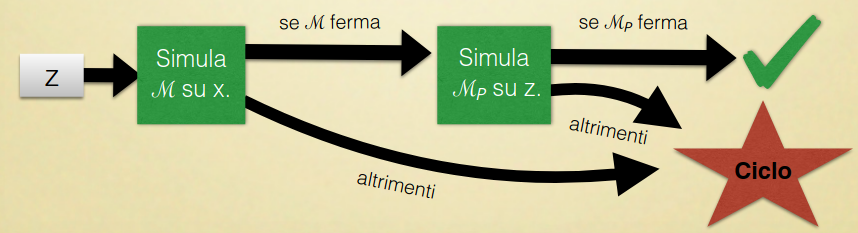
\includegraphics[scale=0.5]{TM_RICE1.png}\\
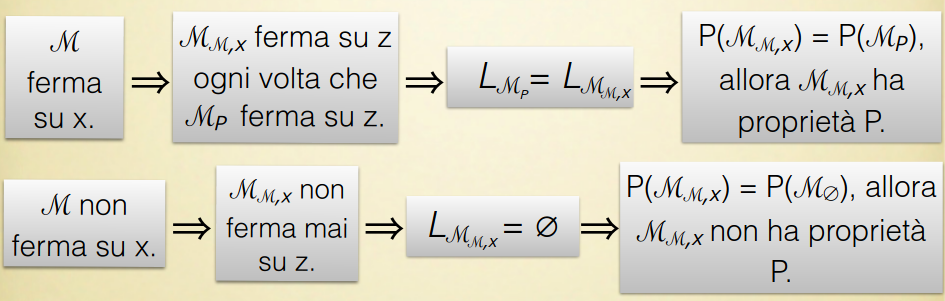
\includegraphics[scale=0.45]{RICE2.png}\\
Se potessimo decidere se $M_{M,x}$ ha la propriet\`a P, potremmo decidere il problema della fermata. Allora, $\{y|y=code(M) e P(M)=1\}$ \`e indecidibile.\\
Abbiamo assunto P($M_{\emptyset}$)=0. Se P($M_{\emptyset}$)=1? In questo caso, ripetiamo lo stesso argomento, ma per la propriet\`a $\neg P$ ("$M$ non ha la propriet\`a P"). Osserva che questo funziona perch\`e: \begin{enumerate}
\item dato che P \`e non-triviale, anche $\neg P$ \`e non-triviale.
\item dato che P($M_{\emptyset}$) = 1, allora $\neg P(M_{\emptyset}) = 1\}$ \`e indecidibile.
\end{enumerate}
Concludiamo che $\{y|y=code(M) \land \neg P(M) = 1\}$ \`e indecidibile. Questo implica che anche $\{y | y=code(M) \land P(M)=1\}$ sia indecidibile.
\end{proof}
NB: lo schema di dimostrazione \`e:
\begin{itemize}
\item Devo dimostrare $A \iff B$
\item Dimostriamo $A \Rightarrow B \land \neg A \Rightarrow \neg B$
\item Che equivale a $A \Rightarrow B \land B \Rightarrow A$
\end{itemize}
\subsection{Proprit\`a decidibili}
Il Teorema di Rice riguarda propriet\`a di \textbf{linguaggio}, non propriet\`a algoritmiche; riguarda funzioni (specifiche), non programmi (implementazioni). Per esempio non possiamo usare il teorema di Rice per derivare l'indecidibilit\`a del problema della fermata (e simili).
In geerale, ci sono tre tipi di propriet\`a riguardo le TM:
\begin{enumerate}
\item \textbf{Propriet\`a di linguaggio}: Quelle non triviali sono indifinibili (teorema di Rice).
\item \textbf{Propriet\`a strutturali}: Queste sono tipicamente decidibili poich\`e si possono verificare staticamente sulla (codifica della) descrizione di TM. (es. $"M\ ha\ 13\ stati"$).
\item \textbf{Propriet\`a comportamentali (o algoritmiche)}: Alcune sono decidibili, altre no, e la classificazione non \`e ovvia (es. $"M\ non\ si\ mouve\ a\ sinistra\ su\ input\ 0101"$).
\end{enumerate}
\section{Tiling}
Mostriamo ora un esmpio di problema non calcolabile in un contesto diverso dalla teoria della computabilit\`a. L'obiettivo generale \`e quello di mostrare che la non-calcolabilit\`a \`e un fenomeno \textbf{pervasivo}, presente in diverse discipline e problemi.\\
Dato un insieme di piastrelle e di regole per metterle insieme, esiste una disposizione del piano che rispetti tali regole?
\subsection{Sistema di Tiling}
Un sistema di tiling \`e costituito da:
\begin{enumerate}
\item Un insieme di piastrelle (tiles) quadrate, per esempio\\
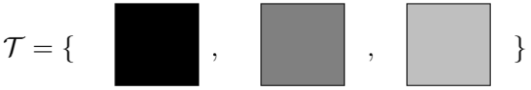
\includegraphics[scale=0.5]{tiling1.png}
\item Un elemento scelto $t_0 \in \tau $ detto piastrella d'origine.
\item Un insieme di $regole di adiacenza$, che specificano quali piastrelle possano essere posate le une accanto alle altre.
\end{enumerate}
\subsection{Tiling}
Il \textbf{tiling} \`e una disposizione delle piastrelle in $\tau$ con le seguenti proprit\`a:
\begin{enumerate}
\item $t_{0}$ si trova nell'angolo in basso a sinistra.
\item Ogni piastrella ha una piastrella sopra e una disposta alla sua destra, senza spazi intermedi.
\item Tutte le regole di adiacenza dono rispettate.
\end{enumerate}
\subsubsection{Esempio}
\begin{center}
L'insieme di piastrelle\\
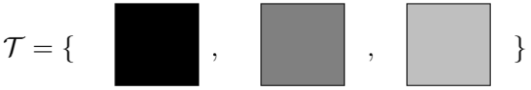
\includegraphics[scale=0.5]{tiling1.png}\\
la piastrella d'origine\\
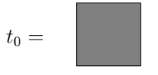
\includegraphics[scale=0.5]{tiling2.png}\\
Regole Orizzontali\\
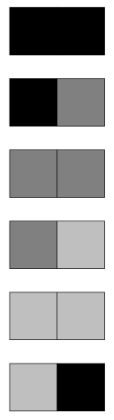
\includegraphics[scale=0.4]{regole_orizzontali.png}\\
Regole Verticali\\
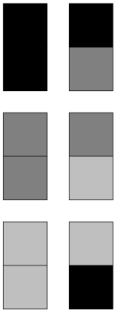
\includegraphics[scale=0.4]{regole_verticali.png}\\
\end{center}
Un tiling per questo sistema \`e per esempio:
\begin{center}
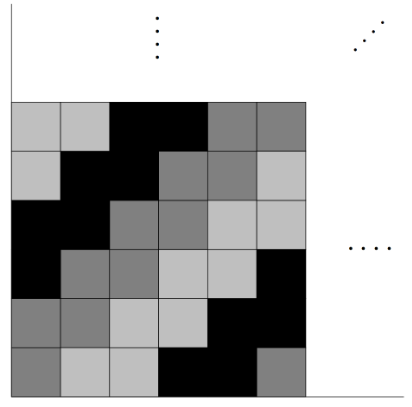
\includegraphics[scale=0.5]{tiling3.png}
\end{center}
\subsection{Il problema del tiling}
Vogliamo analizzare il \textbf{problema del tiling} (tiling problem):
\begin{center}

\textbf{Domanda:}\emph{dato un sistema di tiling, esiste un tiling?}\footnote{1961, Hao Wang.}\\
\textbf{Risposta:}\emph{No.}\footnote{1966, Robert Berger}
\end{center}
Per dimostrare questo, abbiamo bidogno di una definizione formale dei dati del problema.
\subsection{Sistema di tiling, formalmente}
Un \textbf{sistema di tiling} \`e una tupla $\langle \tau, t_0, H, V \rangle$ tale che:
\begin{center}
\begin{enumerate}
\item $\tau$ \`e un insieme di piastrelle.
\item $t_0 \in \tau$ \`e la piastrella d'origine.
\item $H \subset \tau \times \tau$ \`e un insieme di regole di adiacenza orizzontali e $V \subset \tau \times \tau$ \`e un insieme di regole di adiacenza verticali.
\end{enumerate}
\end{center}
Assumiamo il quadrante positivo del piano sia diviso in celle identificate dalle proprie coordinate. Il \textbf{tiling} \`e una funzione $f: \mathbb{N} \times \mathbb{N} \rightarrow \tau$ tale che:
\begin{enumerate}
\item $f(1,1) = t_0$
\item $\forall n,m \in \mathbb{N}.(f(n,m),f(n,m+1)) \in V$
\item $\forall n,m \in \mathbb{N}.(f(n,m),f(n+1,m)) \in V$
\end{enumerate}
\subsection{Problemi di tiling}
Mostreremo che il tiling problem \`e irriconoscibile mostrando che il complemento di $ETH$ si riduce a esso.
\begin{center}
$ETH = \{x \in \sum^{*} | x = code(M) \land M\ ferma\ su\ \epsilon\}$\\
$ETH = \{x \in \sum^{*} | \forall M.x \neq code(M) \lor x = code(M) \land M\ non\ ferma\ su\ \epsilon\}$
\end{center}
Abbiamo visto che $ETH$ \`e indecidibile ma riconoscibile. Quindi come per il problema della fermata e il suo complemento, $ETH^{-}$ deve essere non riconoscibile: altrimenti $ETH$ sarebbe in realt\`a decidibile. Perci\`o, ridurre $ETH^{-}$ al tiling problem implica che il tiling problem non sia riconoscibile da nessuna TM.
La nostra strategia per dimostrare che la non-riconoscibilit\`a  del tiling problem \`e la seguente:
\begin{enumerate}
\item Mostriamo che ogni TM $M$ pu\`o essere trasformata in un sistema di tiling $\tau_{M}$.
\item Questa trasformazione \`e fatta in modo tale per cui \begin{center}
$code(M) \in ETH \iff \not\exists$ un tiling per $\tau_{M}$
\end{center}
\end{enumerate}
Tale corrispondenza riduce $ETH$ al complemento del tiling problem, cos\`i che $ETH^{-}$ si riduce al tiling problem.
\newpage
\section{Teoria della complessit\`a computazionale}
%\subsection{Una lettera di Goedel(1956)}
%Goedel considera una funzione:
%\begin{center}
%$\phi:$ lunghezza $n$ massima della dimostrazione da trovare $\rightarrow$ numero di passi di computazione di una TM
%\end{center}
\subsection{Misurare la complessit\`a}
\begin{center}
$A = \{0^{k}1^{k} | k \geq 0\}$
\end{center}
Programma della TM che decide A:
\begin{enumerate}
\item Leggi l'input e rigetta se trovi uno 0 a destra di un 1.\footnote{$n$ passi.}
\item Fino a che ci sono sia valori 0 che valori 1 sul nastro: scansiona il nastro eliminando un singolo 0 e un singolo 1.\footnote{al pi\`u $n/2 \times n$ passi.}
\item Se rimangono ancora valori 0 o 1, rigetta. Se invece il nastro \`e vuoto, accetta.\footnote{al pi\`u $n$ passi.}
\end{enumerate}
Supponi che l'input abbia lunghezza n. Quanti passi di computazione richiede l'algoritmo?
\subsubsection{Complessit\`a di tempo}
Sia $M$ una TM che si ferma su tutti gli input. La sua \textbf{complessit\`a di tempo} \`e definita come la funzione $f: \mathbb{N} \rightarrow \mathbb{N}$, dove $f(n)$ \`e il massimo numero di passi che $M$ impiega a fermarsi su arbitrari input di lunghezza $n$.\\
Ad esmpio, la TM appena vista ha complessit\`a: $n + (n/2 \times N) + n$\\
Quanto \`e robusto questo metodo di misurare la complessit\`a di un algoritmo?
\begin{enumerate}
\item Dipende dal modello di calcolo.
\item Dipende da cosa intendiamo per 'passi' di computazione.
\item \`E sensibile a variazioni minime (ad es. una sub-routine che richiede un tempo costante, indipendente dall'input).
\item Dipende dalla codifica dell'input e come misuriamo la sua lunghezza.
\end{enumerate}

\subsubsection{Notazione Big-O}
Un modo pi\`u efficace di esprimere la complessit\`a  di un algoritmo \`e usando una notazione che astrae dettagli implementativi poco rilevanti, e fornisce solo una \textbf{stime} significativa del suo tempo di esecuzione.
\begin{center}
date funzioni $f,g: \mathbb{N} \rightarrow \mathbb{N}$ scriviamo $f(n) = O(g(n))$ e diciamo che $g(n)$ \`e un \textbf{bound superiore asintotico} se esistono $c \in \mathbb{N}$, e $m \in \mathbb{N}$ tali che $\forall n. n \geq m. f(n) \leq c \times g(n)$\\In altre parole, $g(n)$ \`e sempre grande almeno quanto $f(n)$ per $n$ sufficientemente grandi e modulo un fattore costante $c$.
\end{center}

\subsubsection{Classi di complessit\`a}
\begin{center}
Data una funzione $f: \mathbb{N} \rightarrow \mathbb{N}$, definiamo \textbf{la classe di complessit\`a}(di tempo) \textbf{TIME(t(n))} come la collezione di tutti i linguaggi decidibili da una TM (deterministica, a un nastro) in te,mpo $O(t(n))$.
\end{center}
Ad esempio il linguaggio A \`e nella classe $TIME(n^{2})$.
\subsection{La classe P}
\begin{center}
P \`e la classe dei linguaggi decidibili da una TM (deterministica, a un nastro) in tempo \textbf{polinomiale}. Ovvero:\\
$P = \bigcup_{k} TIME(n^{k})$
\end{center}
\subsubsection{Perch\`e P?}
Nella pratica dello sviluppo software, un algoritmo che lavora in tempo polinomiale viene solitamente consoderato "ragionevole".\\ Il bound polinomiale pu\`o essere in realt\`a molto alto (es. $O(n^{10})$), ma l'esperienza ci ha rivbelato che, qualora un algoritmo polinomiale \`e conosciuto, \`e solitamente possibile renderlo pi\`u efficiente.\\Un altro aspetto riguarda la codifica, la maggior parte delle codifiche per strutture come grafi, alberi, matrici, automi, ecc. come stringhe richiede tempo polinomiale, e produce una stringa di output di lunghezza polinomiale rispetto all'input.
\subsubsection{Tesi di Church-Turing rafforzata}
Ogni modello di calcolo deterministico fisicamente realizzabile pu\`o essere simulato da una TM (deterministica, su nastro singolo) con overhead al pi\`u polinomiale.\\
$M$ passi di computazione del modello in questione possono essere simulati dalla TM in al pi\`u $O(m^{c})$ passi per una costante $c$.\\
Se vera, la tesi asserisce che la classe P \`e robusta, nel senso di essere invariante rispetto al modello di computazione deterministico scelto.
\subsection{La classe EXP}
P \`e la classe dei linguaggi decidibili in un tempo "ragionevole". \begin{center}
$EXP = \bigcup_{k} TIME(2^{n^{k}})$
\end{center}
EXP \`e la classe dei linguaggi decidibili in un tempo "irragionevole".\\
La classe $EXP$ intutivamente \`e propria degli algoritmi che eseguono un'analisi brute-force, esplorando lo spazio di tutte le possibili soluzioni a un problema.
\subsection{Esempio: PATH}
$PATH = \{\langle G,s,t \rangle |\ G\ grafo\ diretto\ che\ ha\ un\ percorso\ diretto\ da\ s\ a\ t.\}$

\begin{theorem}
PATH \`e in P.
\end{theorem}
\begin{proof}
Considera il seguente algoritmo: 
Su input $\langle G, s,t \rangle$:

\begin{enumerate}
\item Contrassegna il node $s$.
\item Ripeti fino a che nessuno nuovo nodo \`e contrassegnato: [scansiona tutti gli archi di G. Se trovi un arco da nodo a contrassegnato ad uno b non contrassegnato, contrassegna il nodo b.]
\item Se t \`e contrassegnato, accetta. Se no, rigetta.
\end{enumerate}
Analizziamo la complessit\`a: $1$ e $3$ sono chiaramente in P. La subroutine di $2$ \`e in P ed \`e ripetuta al massimo per un numero di nodi di G, quindi $2$ nel suo compleso \`e in P. Perci\`o l'algoritmo \`e in P.
\end{proof}

\subsection{Una nota sulla codifica}
Abbiamo dimostrato che $PATH$ \`e in $P$ assumendo che la complessit\`a venga rispetto al numero di nodi nel grafo. Tuttavia una TM non lavora direttamente su un grafo ma su una sua codifica come stringa di un alfabeto. Per esempio, possiamo codificare un grafo come una matrice di adiacenza, e una matrice di adiacenza come un numero reale.\\ In che modo possiamo essere certi che questo non influenzi la nostra analisi della complessit\`a di PATH? Perch\`e  ciascuna di queste codifiche impiega tempo al pi\`u polinomiale, e modifica la dimensione di questo input di un fattore al pi\`u polinomiale.
\subsection{Altri problemi in P: panoramica}
\begin{enumerate}
\item n \`e primo? S\`i.
\item Il grafo G \`e connesso? S\`i.
\item Data una regex $r$ e la stringa s, $s \in L(r)?$ Probabilmente no (PSPACE-completo).
\item Problema del commesso viaggiatore? Probabilmente no (NP-completo).
\item Dalla posizione P in una fila di s cacchi, quale giocatore ha una strategia vincente? Probabilmente no (PSPACE-completo).
\end{enumerate}
\subsection{La classe NP}
Data una funzione $f: \mathbb{N} \rightarrow \mathbb{N}$, definiamo \textbf{la classe di complessit\`a} (di tempo) \textbf{NTIME(t(n))} come la collezione di tutti i linguaggi decidibili da una TM (non-deterministica, a un nastro) in tempo O(t(n)).
\begin{center}
$NP = \bigcup_k NTIME(n^{k})$
\end{center}

\subsection{Esempio: CLIQUE}
Dato un grafo indiretto, un clique \`e un sotto-grafo dove tutti i nodi sono collegati tra loro da un arco.\\
\begin{center}
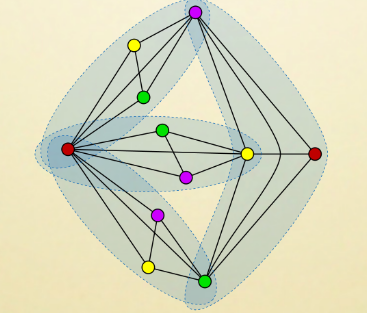
\includegraphics[scale=0.5]{CLIQUE.png}
\end{center}

$CLIQUE = \{\langle G, k \rangle | Il\ grafo\ G\ contiene\ un\ CLIQUE\ di\ k\ nodi.\}$\\
CLIQUE \`e in NP. Ecco una algoritmo non-deterministico polinomiale che lo calcola. Su input $\langle G, k \rangle$

\begin{enumerate}
\item Seleziona non-deterministicamente un sottoinsieme C di k nodi di G.
\item Verifica che G colleghi tutti i nodi di C tramite archi. Se si, accetta. Se no, rigetta.
\end{enumerate}

\subsection{Una caratterizzazione alternativa di NP}
Un linguaggio $A$ \`e \textbf{verificabile} se esiste una $TM\ M$ (che termina sempre, ed accetta o rigetta) con la propriet\`a:
\begin{center}
$w \in A \iff \exists c\ t.c.\ M\ accetta\ \langle w,c \rangle$
\end{center}
Se $M$ lavora in tempo polinomiale, diciamo che A \`e \textbf{verificabile polinomialmente}. Intuitivamente, $c$ \`e un certificato del fatto che $w \in A$. Nota che, se $M$ lavora in tempo polinomiale, pu\`o accedere un certificato di lunghezza al pi\`u polinomiale in w.

\begin{theorem}
Un linguaggio \`e in NP se e solo se \`e verificabile polinomialmente.
\end{theorem}
Idea della dimostrazione.
\begin{proof}
In una direzione, sia M una TM non-deterministica che decide un linguaggio L in tempo polinomiale. Costruiamo un verificatore V polinomiale per L nel seguente modo: Su input $\langle w,c \rangle$:
\begin{enumerate}
\item Simula $M$ su w, trattiamo c come descrizione codificata delle scelte non-deterministiche da prendere nell'albero di computazione di $M$.
\item Se il ramo di computazione esplorato \`e accettante, accetta.
\end{enumerate}
Nella direzione opposta, sia V un verificatore polinomiale per L. Costruiamo una TM $M$ non-deterministica che decide L nel seguente modo: Su input w di lunghezza n:
\begin{enumerate}
\item Seleziona non-deterministicamente una stringa c di lunghezza al pi\`u $n^{k}$.
\item Simula V su input $\langle w, c \rangle$.
\item Se V accetta, accetta. Se no, rigetta.
\end{enumerate}
\end{proof}
\subsection{P vs NP}
\begin{enumerate}
\item P \`e la classe dei linguaggi A per cui la domanda "$w \in A?$" pu\`o essere \textbf{risposta} in maniera efficiente.
\item Np \`e la classe dei linguaggi A per cui la correttezza di una risposta alla domanda "$w \in A?$" pu\`o essere \textbf{verificata} in maniera efficiente.
\end{enumerate}
\subsubsection{Perch\`e Knuth propende per P=NP?}
\begin{enumerate}
\item Gli informatici hanno cercato di dimostrare che P è diverso da NP per lungo tempo, senza successo. Questo é un indizio che il contrario (P = NP) é vero.
\item D’altro canto, altrettante energie sono state impiegate per trovare algoritmi polinomiali per problemi NP, senza successo. É questo un indizio che P é diverso da NP? Secondo Knuth no: questa strategia potrebbe essere sbagliata, un vicolo cieco.
\item Infatti, la dimostrazione che P = NP potrebbe essere non-costruttiva. Dato un problema in NP, un algoritmo polinomiale potrebbe esistere, ma essere incredibilmente complicato, fuori dalla portata umana. Ad esempio, potrebbe essere di complessità O(ng), dove g é il numero di Graham.
\item C’è un precedente significativo per quanto sostiene Knuth: il teorema di Roberston-Seymour, il quale dimostra che un certo problema in teoria dei grafi é in P...ma non dà l’algoritmo polinomiale in sé (e non é chiaro come potremmo
derivarlo in maniera esplicita).
\item In altre parole, secondo Knuth, anche qualora dimostrassimo che P = NP, la dimostrazione sarebbe quasi sicuramente non-costruttiva, e di nessuna utilità pratica.
\end{enumerate}
Perci\`o, in conclusione, Knuth ritiene che P vs NP non sia un problema cos\`i interessante, o quantomeno \`e malposto.


\newpage
\section{Poly reduction}
Siano $L$ e $L'$ linguaggi sull'alfabeto $\sum$ Diciamo che $L$ \`e \textbf{poly (mapping-)riducibile} a $L$, scritto $L' \leq_p L$, se esiste una TM che computa in tempo polinomiale una funzione (totale) $f: \sum^{*} \rightarrow \sum^{*}$ tale che \begin{center}
$x \in L' \iff f(x) \in L$
\end{center}
In altre parole, $L' \leq_p L$ se $L' \leq L$ e la riduzione che lo testimonia \`e computabile in tempo polinomiale.
\subsection{Poly reduction e P}
\begin{theorem}
Se $L' \leq_p L$ e $L \in P$, allora $L' \in P$.
\end{theorem}
\begin{proof}
Da aggiungere. Fatta in classe alla lavagna
\end{proof}
\begin{theorem}
Per $L \in P$, $L^{-} \leq_p L$. 
\end{theorem}
\begin{proof}
Da aggiungere alla lavagna.
$L^{-} \leq_p L$
$x \in L^{-} \iff f(x) \in L$
$x \notin L \iff f(x) \in L$
Problema cos'\`e $f$?
f prende x e calcola se x appartiene ad L (in tempo poly) se s\`i ritorna b non in L , altrimenti a in L. (da correggere)
\end{proof}
\textbf{Domanda}: Se $L \in NP$, $L^{-} \leq_p L$?
\subsection{Formule e soddisfacibilit\`a}
Una formula booleana \`e costuita a partire da variabili $x,y,z,...$, loro negazione $\lnot x, \lnot y, \lnot z,...$(chiamati collettivamente letterali) e combinazioni di letterali tramite congiunzione e disgiunzione ($\land, \lor $). Le variabili possono ricevere valore vero (1) o falso (0), da cui deriviamo il valore di verit\`a dell'intera formula.\\
Esempio: $(\lnot x \lor y) \land (x \lor z)$.\\
Una formula \`e \textbf{soddisfacibile} se esiste un assegnamento di valore alle sue variabili che le dia valore 1. La formula di esempio \`e soddisfacibile, come testimoniato dall'assegnamento $x=1,y=1,z=0$.
\subsubsection{3cnf}
Una formula booleana \`e una \textbf{clausula} se \`e una disgiunzione di variabili (positive o negate).
\begin{center}
$\lnot x \lor y \lor z \lor \lnot z$
\end{center}
Una formula booleana \`e in \textbf{forma normale congiunta (cnf)} se \	e una congiunzione di clausole.
\begin{center}
$(x \lor y) \land (\lnot z \lor z) \land (\lnot z \lor y \lor z \lor \lnot z)$
\end{center}
Una formula booleana \`e \textbf{3cnf} se \`e in cnf e ogni sua clausula contiene esattamente tre letterali.
\subsubsection{3SAT e SAT}
\begin{center}
$SAT = \{\langle F \rangle | F\ formula\ booleana\ soddisfacibile\}$\\
$3SAT = \{\langle F \rangle | F\ formula\ booleana\ 3cnf\ soddisfacibile\}$
\end{center}
Perch\`e sono importanti?\\
\begin{enumerate}
\item ragioni storiche.
\item Ragioni pratiche: molti problemi informatici possono essere formulati come istanze di SAT e 3SAT, ad esmpio constraint programming.
\end{enumerate}
\subsection{3SAT e CLIQUE}
Dimostreremo che $3SAT \leq_p CLIQUE$. La riduzione \`e interessante perch\`e collega problemi all'apparenza molto diversi (uno sulle formule logiche e l'altro sui grafi).
\begin{theorem}
\label{th:10}
3SAT $\leq_p$ CLIQUE
\end{theorem}
\begin{proof}
L'idea della dimostrazione \`e tradurre formule in grafi, dove $f(\langle F \rangle)$ sar\`a costruito in modo tale da 'mimare' il comportamento di variabili e clausole. Un clique in $f(\langle F \rangle)$ corrisponder\`a ad un assegnamento che soddisfa $\langle F \rangle$.
\begin{center}
$\langle F \rangle \in 3SAT \iff f(\langle F \rangle) \in CLIQUE$
\end{center}
\end{proof}

\end{document}



























